\chapter{Lattice Element Types}
\label{c:ele.types}

%---------------------------------------------------------------------------------------------------

This chapter discusses the various types of elements
available in \accellat.
These elements are:
\begin{table}[htb]
\centering
{\tt
\begin{tabular}{llll} \toprule
  {\it Element}    & {\it Section}         & {\it Element}      & {\it Section}       \\ \midrule
  ACKicker         & \ref{s:ackicker}      &  LCavity          & \ref{s:lcavity}     \\
  BeamBeam         & \ref{s:beambeam}      &  Marker           & \ref{s:marker}      \\
  BeginningEle     & \ref{s:begin.ele}     &  Mask             & \ref{s:mask}        \\ 
  Bend             & \ref{s:bend}          &  Match            & \ref{s:match}       \\
  Collimator       & \ref{s:collimator}    &  NullEle          & \ref{s:nullele}     \\
  CrabCavity       & \ref{s:crab}          &  Octupole         & \ref{s:octupole}    \\ 
  Custom           & \ref{s:custom}        &  Patch            & \ref{s:patch}       \\  
  Drift            & \ref{s:drift}         &  Quadrupole       & \ref{s:quadrupole}  \\ 
  EGun             & \ref{s:egun}          &  RFCavity         & \ref{s:rfcavity}    \\ 
  ElSeparator      & \ref{s:elsep}         &  Sextupole        & \ref{s:sextupole}   \\
  Fiducial         & \ref{s:fiducial}      &  Solenoid         & \ref{s:solenoid}    \\
  FloorShift       & \ref{s:floorshift}    &  Taylor           & \ref{s:taylor}      \\
  Foil             & \ref{s:foil}          &  ThickMultipole   & \ref{s:thickmult}   \\
  Fork             & \ref{s:fork}          &  Undulator        & \ref{s:undulator}   \\
  Girder           & \ref{s:girder}        &  UnionEle         & \ref{s:unionele}    \\
  Instrument       & \ref{s:instrument}    &  Wiggler          & \ref{s:wiggler}     \\
  Kicker           & \ref{s:kicker}        &                   &                     \\
  \bottomrule
\end{tabular}
} 
\caption{Table of element types.}
\label{t:particle.classes}
\end{table}

\newpage

%-----------------------------------------------------------------
\section{ACKicker}
\label{s:ackicker}

\begin{example}
  FloorPositionGroup   -> \sref{s:floor.pos.g} Global floor position and orientation.
  LengthGroup          -> \sref{s:length.g} Length and s-position parameters.
  LordSlaveGroup       -> \sref{s:lord.slave.g} Element lord and slave status.
  ReferenceGroup       -> \sref{s:reference.g} Reference energy and species.
  StringGroup          -> \sref{s:string.g} Informational strings.
  TrackingGroup        -> \sref{s:tracking.g} Default tracking settings.
\end{example}

\newpage

%-----------------------------------------------------------------
\section{BeamBeam}
\label{s:beambeam}

\begin{example}
  FloorPositionGroup   -> \sref{s:floor.pos.g} Global floor position and orientation.
  LengthGroup          -> \sref{s:length.g} Length and s-position parameters.
  LordSlaveGroup       -> \sref{s:lord.slave.g} Element lord and slave status.
  ReferenceGroup       -> \sref{s:reference.g} Reference energy and species.
  StringGroup          -> \sref{s:string.g} Informational strings.
  TrackingGroup        -> \sref{s:tracking.g} Default tracking settings.
\end{example}

\newpage

%-----------------------------------------------------------------
\section{BeginningEle}
\label{s:begin.ele}

A \vn{BeginningEle} element must be present as the first element of every tracking branch.
(\sref{s:branch.def}).

Element parameter groups associated with a \vn{BeginningEle} are:
\begin{example}
  LengthGroup          -> \sref{s:length.g}     Length and s-position parameters.
  LordSlaveGroup       -> \sref{s:lord.slave.g} Element lord and slave status.
  StringGroup          -> \sref{s:string.g}     Informational strings.
  ReferenceGroup       -> \sref{s:reference.g}  Reference energy and species.
  FloorPositionGroup   -> \sref{s:floor.pos.g}  Global floor position and orientation.
  TrackingGroup        -> \sref{s:tracking.g}   Default tracking settings.
\end{example}

\newpage

%-----------------------------------------------------------------
\section{Bend}
\label{s:bend}

A \vn{Bend} element represents a dipole bend. Bends have a design bend angle and bend radius
which determines the location of downstream elements as documented in \sref{s:machine.coords}.
The actual bending strength that a particle feels can differ from the design value as detailed
below.

\noindent\rule{\linewidth}{0.5pt}
Element parameter groups associated with a \vn{BeginningEle} are:
\vskip 0.7ex
\begin{example}
  AlignmentGroup     -> Element position/orientation shift. \sref{s:align.g} 
  ApertureGroup      -> Vacuum chamber aperture. \sref{s:aperture.g} 
  BMultipoleGroup    -> Magnetic multipoles. \sref{s:bmultipole.g} 
  BendGroup          -> Bend element parameters. \sref{s:bend.g} 
  EMultipoleGroup    -> Electric multipoles. \sref{s:emultipole.g} 
  FloorPositionGroup -> Global floor position and orientation. \sref{s:floor.pos.g} 
  LengthGroup        -> Length and s-position parameters. \sref{s:length.g} 
  LordSlaveGroup     -> Element lord and slave status. \sref{s:lord.slave.g} 
  MasterGroup        -> Contains field_master parameter. \sref{s:master.g} 
  ReferenceGroup     -> Reference energy and species. \sref{s:reference.g} 
  StringGroup        -> Informational strings. \sref{s:string.g} 
  TrackingGroup      -> Default tracking settings. \sref{s:tracking.g} 
\end{example}
\noindent\rule{\linewidth}{0.5pt}

\begin{figure}[ht]
  \centering 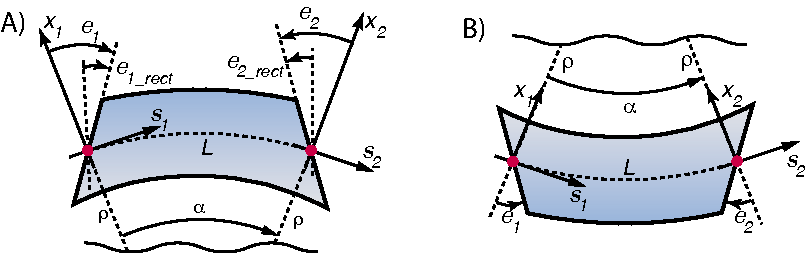
\includegraphics{bend.pdf} 
\caption[Bend geometry]{
Bend geometry. Red dots are the entry and exit points that define the origin for the
coordinate systems at the entry end $(s_1, x_1)$ and exit ends $(s_2, x_2)$ respectively. 
In the figure, the angle \vn{alpha} is denoted $\alpha$ and the radius
\vn{rho} is denoted $\rho$.
A) Bend geometry with positive bend angle. For the geometry shown, 
\vn{g}, \vn{angle}, \vn{rho}, \vn{e1}, \vn{e2}, \vn{e1_rect}, and \vn{e2_rect} are all positive.
B) Bend geometry with negative bend angle. For the geometry shown, 
\vn{g}, \vn{angle}, \vn{rho}, \vn{e1}, \vn{e2}, \vn{e1_rect}, and \vn{e2_rect} are all negative.
Note: The figures are drawn for zero \vn{ref_tilt} where the rotation axis is parallel to the 
$y$-axis. 
}
\label{f:bend}
\end{figure}

\vn{BendGroup} parameters are:
  \begin{description}
  %
  \index{angle}
  \item[angle] \Newline
The total design bend angle. A positive \vn{angle} represents a
bend towards negative $x$ as shown in \fig{f:bend}.
  %
  \index{bend_field}
  \item[bend_field] \Newline
The \vn{bend_field} parameter is the design magnetic bending field which determines the reference orbit
and the placement of lattice elements downstream from the bend. The actual (``total'') field is
a vector sum of
\vn{bend_field} plus the value of the \vn{Bn0}  and \vn{Bs0} multipoles. If \vn{tilt0} and \vn{Bs0}
are zero, the actual field is
\begin{example}
  B-field (total) = bend_field + Bn0
\end{example}
See the discussion of \vn{g} and \vn{Kn0} below for more details.
  %
  \index{e1}\index{e2}
  \item[e1, e2] \Newline
The values of \vn{e1} and \vn{e2} gives the rotation angle of the entrance and exit pole faces
respectively with respect to the radial $x_1$ and $x_2$ axes as shown in \fig{f:bend}.
Zero \vn{e1} and \vn{e2} gives a wedge shaped magnet (\fig{f:sbend}).
Also see \vn{e1_rect} and \vn{e2_rect}. The relationship is
\begin{example}
  e1 = e1_rect + angle/2
  e2 = e2_rect + angle/2
\end{example}

Note: The correspondence between \vn{e1} and \vn{e2} and the corresponding parameters used in the
SAD program \cite{b:sad} is:
\begin{example}
  e1(AccelLat) =  e1(SAD) * angle + ae1(SAD)
  e2(AccelLat) =  e2(SAD) * angle + ae2(SAD)
\end{example}
  %
  \item[e1_rect, e2_rect]
Face angle rotations like \vn{e1} and \vn{e2} except angles are measured with respect to 
fiducial lines that are parallel to each other and rotated by \vn{angle}/2 from the radial
$x_1$ and $x_2$ axes as shown in \fig{f:sbend}. 
Zero \vn{e1_rect} and \vn{e2_rect} gives a rectangular magnet shape.
  %
  \index{exact_multipoles}
  \item[exact_multipoles] \Newline
The \vn{exact_multipoles} switch can be set to one of:
\begin{example}
  off                 ! Default
  vertically_pure    
  horizontally_pure  
\end{example}
This switch determines if the multipole fields, both magnetic and electric, and including the
\vn{k1} and \vn{k2} components, are corrected for the finite curvature of the reference orbit in a
bend. See \sref{s:field.exact} for a discussion of what \vn{vertically} pure versus
\vn{horizontally} pure means. Setting \vn{exact_multipoles} to \vn{vertically_pure} means that the
individual $a_n$ and $b_n$ multipole components are used with the vertically pure solutions
\begin{equation}
  \bfB = \sum_{n = 0}^\infty \left[ \frac{a_n}{n+1} \nabla \phi_n^r + \frac{b_n}{n+1} \nabla \phi_n^i \right], \qquad
  \bfE = \sum_{n = 0}^\infty \left[ \frac{a_{en}}{n+1} \nabla \phi_n^i + \frac{b_{en}}{n+1} \nabla \phi_n^r \right]
\end{equation}
and if \vn{exact_multipoles} is set to \vn{horizontally_pure} the horizontally pure solutions
$\psi_n^r$ and $\psi_n^i$ are used instead of the vertically pure solutions $\phi_n^r$ and
$\phi_n^i$.
  %
  \index{fint1}\index{fint2}\index{hgap1}\index{hgap2}
  \item[fint1, fint2, hgap1, hgap2] \Newline
The field integrals for the entrance pole face is given by the product of the \vn{fint} and
\vn{hgap} parameters with \vn{hgap} being the half gap between poles at the entrance face
\begin{equation}
  F_{H1} \equiv F_{int1} \, H_{gap1} = \int_{pole} \! \! ds \, \frac{B_y(s) \, (B_{y0} - B_y(s))}
  {2 \, B_{y0}^2}
  \label{fsbbb}
\end{equation}
For the exit pole face there is a similar equation using \vn{fint2} and \vn{hgap2} which defines
$F_{H2}$. In the above equation $B_{y0}$ is the field in the interior of the dipole. The values of
\vn{fint1}, \vn{fint2}, \vn{hgap1}, and \vn{hgap2} are never used in isolation when tracking. Only
the values for $F_{H1}$ and $F_{H2}$ matter.
That is, to have an effect, both \vn{fint} and \vn{hgap} (or \vn{fintx} and \vn{hgapx}) must be non-zero.

Note: The SAD program uses \vn{fb1+f1} for the entrance fringe and \vn{fb2+f1} for the exit
fringe. The correspondence between the two is
\begin{example2}
  \(F_{H1}\) = fint  * hgap  = (fb1 + f1) / 12
  \(F_{H2}\) = fintx * hgapx = (fb2 + f1) / 12
\end{example2}

\index{Enge function}
\vn{fint} and \vn{hgap} can be related to the Enge function which is sometimes used to model the
fringe field. The Enge function is of the form
\begin{equation}
  B_y(s) = \frac{B_{y0}}{1 + \exp[P(s)]}
\end{equation}
where
\begin{equation}
  P(s) = C_0 + C_1 \, s + C_2 \, s^2 + C_3 \, s^3 + \, \ldots
\end{equation}
The $C_0$ term simply shifts where the edge of the bend is. If all the $C_n$ are zero except for
$C_0$ and $C_1$ then
\begin{equation}
  C_1 = \frac{1}{2 \,H_{gap} \, F_{int}}
\end{equation}
  %
  \item[fiducial_pt] \Newline
The \vn{fiducial_pt} parameter sets a fiducial point which can be used to keep the shape of the bend
constant when, in a program, the parameters \vn{rho}, \vn{g}, \vn{b_field} or \vn{angle} are varied.
Varying these parameters typically happens when doing machine design. Using a fiducial point can be
helpful when designing a machine usin bend magnets that already exist.

The \vn{fiducial_pt} parameter
has four possible settings:
\begin{example}
  none          ! No fiducial point (default).
  entrance_end  ! The entrance point is the fiducial point.
  center        ! The center of the reference curve is the fiducial point.
  exit_end      ! The exit point is the fiducial point.
\end{example}
With \vn{fiducial_pt} set to \vn{none} (the default). The bend shape is not held constant. With the
other three settings, the bend shape will be held constant as discussed in \sref{s:bend.fiducial}.
With \vn{fiducial_pt} set to \vn{entrance_end}, the reference trajectory at the entrance end is held
fixed in both position and orientation with respect to the bend face and \vn{g}, \vn{l} and \vn{e2},
along with the other depdendent parameters, are adjusted to both give the desired change in what was
varied (which is one of \vn{rho}, \vn{g}, \vn{b_field} or \vn{angle}) and to keep the shape of the
bend unchanged. See \fig{f:bend.fid1}. Similarly, if \vn{fiducial_pt} is set to \vn{center}, the
center of the reference trajectory is held fixed in both position and orientation and if
\vn{fiducial_pt} is set to \vn{exit_end}, the exit point is held fixed in both position and
orientation.
  %
  \index{g}\index{rho}
  \item[g, rho] \Newline
The design bending radius which determines the reference coordinate system is \vn{rho} (see
\sref{s:ref}). \vn{g} = \vn{1/rho} is the ``bend strength'' and is proportional to the design
dipole magnetic field. \vn{g} is related to the design magnetic field \vn{bend_field} via
\begin{equation}
  \text{g} = \frac{q}{p_0} \, \text{bend_field} 
  \label{gqpb}
\end{equation}
where $q$ is the charge of the reference particle and $p_0$ is the reference momentum. It is
important to keep in mind that changing \vn{g} will change the design orbit (\sref{s:coords.3}) and
hence will move all downstream lattice elements in space.

The total bend strength felt by a particle is the vector sum of \vn{g} plus the zeroth order
magnetic multipole. If the multipole \vn{tilt0} and \vn{Ks0} is zero, the total bend strength is
\begin{example}
  g_total = g + Kn0
\end{example}
Changing the multipole strength \vn{Kn0} or \vn{Ks0} leaves the design orbit and the positions of
all downstream lattice elements
unchanged but will vary a particle's orbit. One common mistake when designing lattices is to vary
\vn{g} and not \vn{Kn0} which results in downstream elements moving around. See \Sref{s:ex.chicane}
for an example.

Note: A positive \vn{g}, which will bend particles and the reference orbit in the $-x$ direction
represents a field of opposite sign as the field due a positive \vn{hkick}.
  %
  \index{h1}\index{h2}
  \item[h1, h2] \Newline
The attributes \vn{h1} and \vn{h2} are the curvature of the entrance and exit pole faces.
  %
  \index{L}\index{L_chord}\index{L_arc}\index{L_sagitta}
  \item[L, L_arc, L_chord, L_sagitta]  \Newline
The \vn{L} parameter is the arc length of the reference trajectory through the bend.

\vn{L_chord} is the chord length from entrance point to exit point.
The \vn{L_sagitta} parameter is the sagitta length (The sagitta is the distance
from the midpoint of the arc to the midpoint of the chord). \vn{L_sagitta} can be negative and will have
the same sign as the \vn{g} parameter.
  %
  \item[L_rectangle] \Newline
The \vn{L_rectangle} parameter is the ``rectangular'' length defined to be the distance between the
entrance and exit points. The coordinate system used for the calculation is defined by the setting
of \vn{fiducial_pt}. \fig{f:rbend} shows \vn{l_rectangle} for \vn{fiducial_pt} set to
\vn{entrance_end} (the coordinate system corresponds to the entrance coordinate system of the bend).
In this case, and in the case where \vn{fiducial_pt} is set to \vn{exit_end}, the rectangular
length will be $\rho \sin\alpha$. If \vn{fiducial_pt} is set to \vn{none} or \vn{center},
\vn{l_rectangle} is the same as the chord length.
  %
  \index{ref_tilt}
  \item[ref_tilt] \Newline
The \vn{ref_tilt} attribute rotates a bend about the longitudinal axis at the entrance face of the
bend. A bend with \vn{ref_tilt} of $\pi/2$ and positive \vn{g} bends the element in the $-y$
direction (``downward''). See \fig{f:tilt.bend}. It is important to understand that \vn{ref_tilt},
unlike the \vn{tilt} attribute of other elements, bends both the reference orbit along with the
physical element. Note that the MAD \vn{tilt} attribute for bends is equivalent to the \bmad
\vn{ref_tilt}. Bends in \bmad do not have a \vn{tilt} attribute.

Important! Do not use \vn{ref_tilt} when doing misalignment studies for a machine. Trying to misalign
a dipole by setting \vn{ref_tilt} will affect the positions of all downstream elements! Rather, use the
\vn{tilt} parameter.
  \end{description}

%---------------


The attributes \vn{g}, \vn{angle}, and \vn{L} are mutually dependent. If any two are specified for
an element \bmad will calculate the appropriate value for the third.

In the local coordinate system (\sref{s:ref}), looking from ``above'' (bend viewed from positive
$y$), and with \vn{ref_tilt} = 0, a positive \vn{angle} represents a particle rotating clockwise. In
this case. \vn{g} will also be positive. For counterclockwise rotation, both \vn{angle} and \vn{g}
will be negative but the length \vn{l} is always positive. Also, looking from above, a positive
\vn{e1} represents a clockwise rotation of the entrance face and a positive \vn{e2} represents a
counterclockwise rotation of the exit face. This is true irregardless of the sign of \vn{angle} and
\vn{g}. Also it is always the case that the pole faces will be parallel when
\begin{example}
  e1 + e2 = angle
\end{example}

Example bend specification:
\begin{example}
  @ele b03w = Bend(l = 0.6, kn1 = 0.003)
\end{example}

\newpage

%-----------------------------------------------------------------
\section{Collimator}
\label{s:collimator}


%-----------------------------------------------------------------
\section{CrabCavity}
\label{s:crab}


%-----------------------------------------------------------------
\section{Custom}
\label{s:custom}


%-----------------------------------------------------------------
\section{Drift}
\label{s:drift}


%-----------------------------------------------------------------
\section{EGun}
\label{s:egun}


%-----------------------------------------------------------------
\section{ElSeparator}
\label{s:elsep}


%-----------------------------------------------------------------
\section{Fiducial}
\label{s:fiducial}


%-----------------------------------------------------------------
\section{FloorShift}
\label{s:floorshift}


%-----------------------------------------------------------------
\section{Foil}
\label{s:foil}


%-----------------------------------------------------------------
\section{Fork}
\label{s:fork}


%-----------------------------------------------------------------
\section{Girder}
\label{s:girder}


%-----------------------------------------------------------------
\section{Instrument}
\label{s:instrument}


%-----------------------------------------------------------------
\section{Kicker}
\label{s:kicker}


%-----------------------------------------------------------------
\section{LCavity}
\label{s:lcavity}


%-----------------------------------------------------------------
\section{Marker}
\label{s:marker}


%-----------------------------------------------------------------
\section{Mask}
\label{s:mask}


%-----------------------------------------------------------------
\section{Match}
\label{s:match}


%-----------------------------------------------------------------
\section{NullEle}
\label{s:nullele}


%-----------------------------------------------------------------
\section{Octupole}
\label{s:octupole}


%-----------------------------------------------------------------
\section{Patch}
\label{s:patch}


%-----------------------------------------------------------------
\section{Quadrupole}
\label{s:quadrupole}


%-----------------------------------------------------------------
\section{RFCavity}
\label{s:rfcavity}


%-----------------------------------------------------------------
\section{Sextupole}
\label{s:sextupole}


%-----------------------------------------------------------------
\section{Solenoid}
\label{s:solenoid}


%-----------------------------------------------------------------
\section{Taylor}
\label{s:taylor}


%-----------------------------------------------------------------
\section{ThickMultipole}
\label{s:thickmult}


%-----------------------------------------------------------------
\section{Undulator}
\label{s:undulator}


%-----------------------------------------------------------------
\section{UnionEle}
\label{s:unionele}


%-----------------------------------------------------------------
\section{Wiggler}
\label{s:wiggler}


